\documentclass[a4paper,12pt]{article}

\usepackage{graphicx}
\usepackage{algorithm}
\usepackage{algorithmic}
\usepackage{amsmath}
\usepackage[usenames,dvipsnames]{color}
\usepackage{listings}

\definecolor{Brown}{cmyk}{0,0.81,1,0.60}
\definecolor{OliveGreen}{cmyk}{0.64,0,0.95,0.40}
\definecolor{CadetBlue}{cmyk}{0.62,0.57,0.23,0}
\definecolor{orange}{rgb}{0.7,0.3,0}
\definecolor{graycolor}{rgb}{0.2,0.2,0.2}
\definecolor{lightlightgray}{gray}{0.9}

\lstset{
language=C,                             % Code langugage
basicstyle=\ttfamily,                   % Code font, Examples: \footnotesize, \ttfamily
keywordstyle=\color{OliveGreen},        % Keywords font ('*' = uppercase)
commentstyle=\color{graycolor},              % Comments font
stringstyle=\color{orange},
numbers=left,                           % Line nums position
numberstyle=\tiny,                      % Line-numbers fonts
stepnumber=1,                           % Step between two line-numbers
numbersep=5pt,                          % How far are line-numbers from code
backgroundcolor=\color{lightlightgray}, % Choose background color
frame=none,                             % A frame around the code
tabsize=2,                              % Default tab size
captionpos=b,                           % Caption-position = bottom
breaklines=true,                        % Automatic line breaking?
breakatwhitespace=false,                % Automatic breaks only at whitespace?
showspaces=false,                       % Dont make spaces visible
showtabs=false,                         % Dont make tabls visible
morekeywords={__global__, __device__, __global, __kernel},  % CUDA specific keywords
}


\begin{document}

\title{An efficient GPU framwork for Image Processing}
\author{Per Karlsson}
\date{September 2014}
\maketitle

\setlength\parindent{0pt}

\begin{abstract}
\noindent
To be added

\end{abstract}


\tableofcontents
\setcounter{tocdepth}{2}

\section{Introduction}
\subsection{Background}
\subsubsection{Image Processing}
An image can be seen as a mathematical function $i(x,y)$ where $x$ and $y$ are the spatial coordinates and the output is a color at position $(x,y)$. If the color has a discrete quantities and the total image has a finite element of samples, it is called a \emph{Digital Image}. The samples each has a unique spatial coordinate and are referred to as \emph{pixels}. The field of \emph{Digital Image Processing} refers to processing a digital image and its pixels. Every time Image Processing is mentioned in this theis, it is assumed that it refers to Digital Image Processing. 
\newline

It is not obvious what 
\begin{figure}[ht!]
\centering
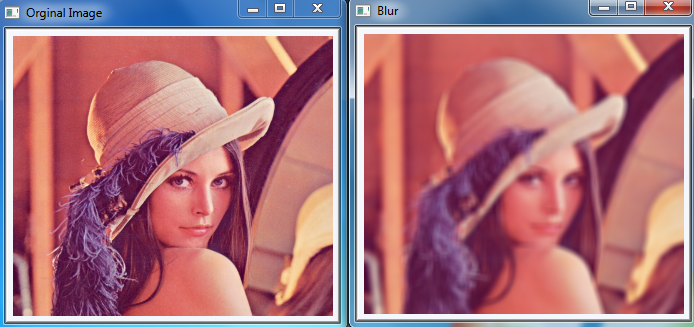
\includegraphics[width=80mm]{img/lena.png}
\caption{A blur algorithm is applied on an input image and produces a blurred output image.}
\label{lena}
\end{figure}

\begin{figure}[ht!]
\centering
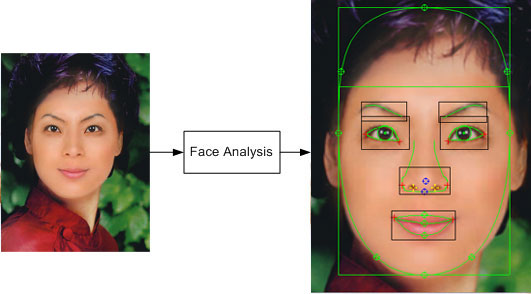
\includegraphics[width=80mm]{img/feature.jpg}
\caption{The input image of a face is analyzed to find features such as nose, mouth and eyes.}
\label{feature}
\end{figure}

\subsection{Purpose}

\subsection{Limitations}

As discussed in the previous chapter, there are different categories in image processing. This thesis will focus on the case where an input image is used to produce an output image. Mainly because it is hard to generalize things like feature extraction across all GPU environments. The framework is instead going to support algorithms where an arbitrary number of input images are going to produce an arbitrary number of output images. The number of input images and output images do not have to match. The framework need to support multipass algorithms where multiple GPU programs are being called sequentionally and where the output of one program can be the input of the following one. The framework is going support images with one to four channels of colors and where the data has either floating point precision or is of the unsigned byte type (often referred to as unsigned char).
\newline

The framework is going to support the following GPU computing environemnts:

\begin{itemize}
\item{{\bf CUDA} - NVIDIA}
\item{{\bf OpenCL} - Khronos Group}
\item{{\bf GLSL} - OpenGL Shading Language}
\end{itemize}

CUDA and OpenCL are the two most common choices today in the world of general-purpose GPU computing. Before OpenCL and CUDA, people used programmable shaders in 3D graphics libraries such as OpenGL and DirectX to perform image processing on the GPU. Since DirectX and their HLSL shading language and Direct Compute environment only are support on Microsoft Windows systems, they are not included in the framework of this thesis as it aims to be flexible and cross-platorm (supporting both Linux, Mac and Windows systems).

\subsection{Method}

To get more knowledge and experience about the different GPU environments, the first phase of the thesis work will involve individual work with CUDA, OpenCL and GLSL. The middle phase of the project will be the implementation of all the software components. This will be an iterative process. First a prototype will be created and after feedback from a supervisor and other people involved in the project, a second improved version will be implemented. For every feature added in the backend library, a unit test is added to test the feature and all its cases. The last part of the thesis work will involve testing and more specifically, testing with practical image processing problems. The testing part serves the purpose of benchmarking speed, testing how practical the framework is and examine if any GPU environment is better than the others in terms of functionality.

\subsection{Structure}
This thesis is going to be structed the following way:

\begin{itemize}
\item{\bf{Introduction}}
\item{\bf{Parallel Environments}}
\item{\bf{Implementation}}
\item{\bf{Test cases}}
\item{\bf{Result}}
\item{\bf{Discussion}}
\end{itemize}




\section{Parallel Environments}
\subsection{GLSL}

\subsubsection{OpenGL}

OpenGL is a cross-platform API created in 1992. It has been an industry-standard ever since where the major decisions are made by the OpenGL Architecture Review Board, ARB. ARB was created by Silicon Graphics in 1992 and contained representatives from SGI, Intel, Microsoft, Compaq, Digital Equipment Corporation, Evans \& Sutherland and IBM. Later on, companies such as 3Dlabs, Apple, ATI, Dell, IBM, Intel, nVIDIA and Sun Microsystems were added. OpenGL shares many characteristics of a previous API called Iris GL. It is designed in such way that it aimes to the be lowestlevel interface for accessing graphics hardware but still provide hardware independence. OpenGL is supported in PC, Mac and Unix-systems.

\begin{figure}[ht!]
\centering
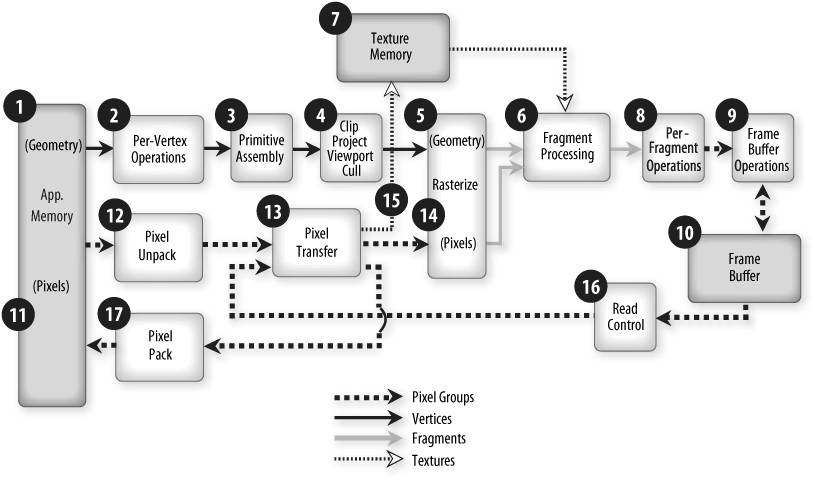
\includegraphics[width=100mm]{img/fixed-gl.jpg}
\caption{The OpenGL pipeline until version 1.5 had fixed functionality.}
\label{glfixed}
\end{figure}

Figure \ref{glfixed} shows the overview of the complete OpenGL pipeline until version 1.5. It was said to have fixed functionality because every OpenGL implementation is required to have the same functionality. The set of operations and how they were applied were defined by the fixed OpenGL specification. Step number 6 in Figure \ref{glfixed}, the Fragment Processing, is where each fragment gets its final value. A fragment can be thought of as the data needed to shade the pixel and the data to decide if the fragment is to be displayed as a pixel (need information about depth, alpha and so on). The fixed fragment stage could only handle tasks such as interpolating color values, texture mapping and fog. 

\subsubsection{The shading language}

In version 2.0, OpenGL introduced GLSL, the OpenGL shading language. With the OpenGL shading language, the fixed functionality stages for vertex and fragment processing (Step 2 and 6 in Figure \ref{glfixed}) could now be customized and programmed. It is still possible to do everything that the previous fixed pipeline supported but it also gives the software developer the opportunity to alone control the output. The programs written in GLSL are called OpenGL shaders, either vertex shader or fragment shader. The OpenGL Shading Language is a high-level procedural language based on C and C++ sytax and flow control. Vector and matrix types/operations is natively supported together with a set of  math functions commonly used in graphics shading.
\newline

\subsubsection{Shaders}

\begin{figure}[ht!]
\centering
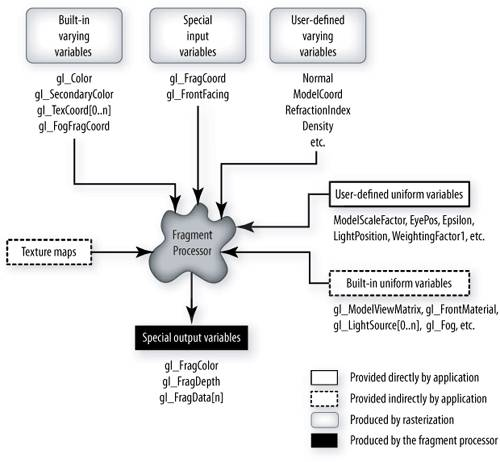
\includegraphics[width=100mm]{img/frag-gl.jpg}
\caption{The input and outputs of a GLSL fragment shader.}
\label{glfrag}
\end{figure}

Shaders are compiled from an input source of text at runtime. They are later linked to an OpenGL program and are then executable. In image processing, only the fragment shader is of importance. In a fragment shader, any image processing algorithm can be applied on an input image. A fragment shader operates on one fragment at a time. Fragment shaders must be written in such way that the can operator simulationeusly. When a fragment shader is being executed, it has no knowledge about other fragments and their data. 
\newline

Figure \ref{glfrag} shows the inputs and output of a fragment processor. Some variables are built-in, specified by the OpenGL implementation. There is a notion of varying and uniform variables. Uniform variables are, as the name suggests, uniform accross all shaders. Varying variables are defined per vertex in the vertex shader. Before processing each fragment, the hardware interpolates the geometry and gives the fragment shader the correct varying attributes. An example of a varying attribute would be where one wants to output a texture on some sort of geometry. The texture coordinates would then be defined at each vertex. In the later processing of the fragment shader, these texture coordinate are interpolated and can now be used to do texture lookups. 

\renewcommand{\lstlistingname}{Code}
\begin{lstlisting}[caption= Example of adding two images in GLSL, label=glsl1]
uniform sampler2D texture0;
uniform sampler2D texture1;

uniform float scale;
varying vec2 texcoord;

void main()
{
    gl_FragData[0] = scale * (
        texture2D(texture0, texcoord) + 
        texture2D(texture1, texcoord));

}
\end{lstlisting}

Code \ref{glsl1} shows an example of fragment shader in GLSL that adds two images together. The images have been converted to OpenGL textures, \texttt{texture0} and \texttt{texture1}. The function \texttt{texture2D} together with the varying variable \texttt{texcoord} is used to fetch the data from a texture. The value is multiplied with the uniform value \texttt{scale} (same for all fragments) and finally written to the framebuffer through the built-in \texttt{gl\_FragData}. Syntax is similar to a C program and every fragment shader needs a \texttt{main} function.

\newpage
\subsection{CUDA}

The CUDA architechure was released for the first time in 2006 to make it easier to perform general purpose GPU-computing. Unlike previous methods that had to get around the old pipeline with vertex and fragment shaders, CUDA allowed every aritmethic logic unit on the chip to be controlled by a CUDA program. Another important feature was the possibility to read and write to arbitrary memory address on the GPU in comparison to previous methods that required textures as storage. The hardware was still in charge of memory caching but CUDA also exposed a software managed cache called shared memory. CUDA programs are written in the CUDA C language, a language very close to the C language with the exception of a small number of keywords added for special features in the CUDA architecture.  

\subsubsection{Blocks and threads}

In the CUDA architechure, threads are single execution units that run kernels on the GPU. They are similar to CPU threads but the typically there are a lot more of them on the GPU. The threads are divided into thread blocks. Threads within a thread block can communicate with each others. The number of blocks and threads per block is decided by the developer when the kernel is called. The grid of block can be one, two or three dimensional. The maximum number of blocks and threads per block is decided by the GPU and its hardware. A CUDA kernel is executed simulatenously by warps. A warp consists of threads within a block. Typically each warp has the size of 32 threads, where actions like memory read and writes are performed in half-warps. 
\newline

\begin{figure}[ht!]
\centering
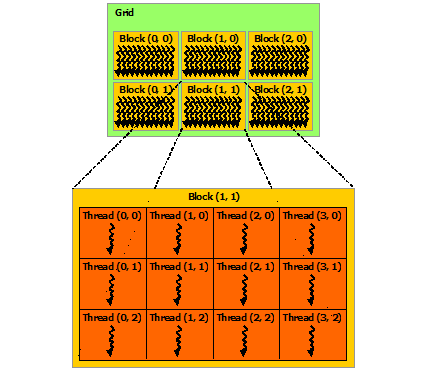
\includegraphics[width=80mm]{img/grid-of-thread-blocks.png}
\caption{CUDA threads divided into blocks of threads.}
\label{cudablockthreads}
\end{figure}

\renewcommand{\lstlistingname}{Code}
\begin{lstlisting}[caption= Example of vector addition in CUDA, label=cuda1]
__global__ void VectorAddition(float * A, 
                               float * B, 
                               float * C)
{
    int i = blockIdx.x * blockDim.x + threadIdx.x;
    int j = blockIdx.y * blockDim.y + threadIdx.y;
    int idx = i + j * gridDim.x * blockDim.x;
    C[idx] = A[idx] + B[idx];
}
\end{lstlisting}

When a thread is executing a kernel, there are built-in variables to access information of which block the thread belongs to and the local thread index in the actual block. This is often used to know where to read and write in a global array. Code \ref{cuda1} shows an example of a simple CUDA kernel performing a vector addition. The keyword \texttt{\_\_global\_\_} is used to tell the compiler that the function is a CUDA kernel. The variables \texttt{blockIdx}, \texttt{threadIdx}, \texttt{gridDim} and \texttt{blockDim} are automatically built-in in a CUDA kernel and can be accessed at any time. \texttt{blockIdx} and \texttt{threadIdx} are of the type \texttt{uint3}, where each value represent an index in the corresponding dimension. \texttt{blockIdx} is the index of the block in the total grid of launched blocks and \texttt{threadIdx} is the thread index within the block. Both \texttt{gridDim} and \texttt{blockDim} are of the type \texttt{dim3} and are constant in all threads (not possible to launch a kernel with different block sizes).

\subsubsection{Memory hierarchy}
\begin{figure}[ht!]
\centering
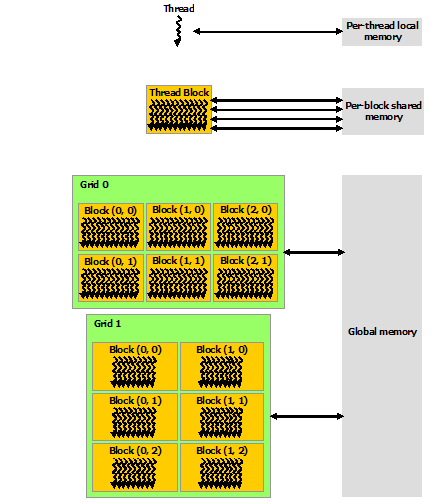
\includegraphics[]{img/memory-hierarchy.png}
\caption{Different CUDA memory spaces}
\label{cudamemoryhierarchy}
\end{figure}
There are differnet memory spaces in the CUDA architechure as can be seen in Figure \ref{cudamemoryhierarchy}. Each thread has a local and private memory space. All the threads in a block can share a memory space, called shared memory. Shared memory is on-chip and is divided into different banks. Reading from shared memory in warp of threads is just as fast as reading from a register as long as there are no bank conflicts. Each bank conflict results in a serialized read from the shared memory. Worst case scenario is when all threads in a warp only read from one bank in the shared memory. The shared memory read then becomes a lot slower then the regular global memory. Global, constant and texture memory can all all be accessed by all threads. Constant and texture memory are only used in certain cases where the global memory is the common choice for storing data. The texture memory space is cached to that a texture fetch only cost a GPU device memory read on a cache miss, otherwise it only costs a read from the texture cache. Texture cache is optimized for 2D spatial locality. If desired, one also gets an automatic linear interpolation when reading from the texture space. Constant memory is a read-only memory space. All the threads of a half-warp read from constant memory just as fast as from a register as long as all the threads read from the same address. The cost scales linearly with the number of different addressed read by the threads. For example, the worst case would be if an array would be stored in the constant memory space and each thread in an executing half-warp needs an unique value in this array. The commonly used global memory space is capable of reading 4, 8 and 16 bytes of memory into registers in one single instruction. The most efficient global memory reads are when all threads in a half-warp reads from continous memory in a coalesced read of 64, 128 or 256 bytes. It is impossible for a thread to know if the current value in the global memory  has been updated or not if a kernel is reading and writing to the same global memory. CUDA supports atomic operations but they are usually slow and a common technique is to have to different buffers allocated, one to read from and one to write to.




\subsection{OpenCL}

\subsubsection{Standarized framework for heterogeneous systems}

OpenCL is a parallel programming framework designed to fit heterogeneous systems where one can expect a range of different computing architechures. One example of a program on a heterogeneous system would be a program where some parts of the computations and setups are done on the CPU and the rest on the GPU. OpenCL also supports parallel programming for homogeneous systems. In a case where one has a multi-core CPU, OpenCL could be used to in such way to have one thread control the state of the program while the rest of the threads performs a computation of some sort and later sync with the main thread.
\newline

OpenCL is standarized by the Khronos Group, the same group in charge of well known OpenGL standarization. The group consits of people from many different companies in the industry such as AMD, nVIDIA, intel, Apple, Samsung. This is seen as a positive thing as they all decide the direction the group is taking. It also makes sure the framework compatible for different system and platforms. One of the goals of OpenCL is to be as flexible as possible.
\newline

\subsubsection{The OpenCL C language}
OpenCL can be used in any parallel environent as long as the OpenCL compiler and runtime library is implemented. This means, when writing the parallel code, a software developer do not have have care about operating system, processors and memory types. The OpenCL C language is very similar to the regular C language. It is focused around computations and some features are added on top of the C language to simplfy things, like SIMD vector operations and multiple memory hierarhies. Other features, such as printing, have been removed as they are not as useful in computing and hard to implement on all platforms. The program calling the OpenCL code can be written in either C or C++ as it will be using the OpenCL runtime library. 
\newline

The notion of host is often used in standard and offical OpenCL literature. The host refers to the environment where the OpenCL code is called from (not executed). This is the CPU in almost all of the cases. An OpenCL device is the environment where the OpenCL is executed. This can be the GPU, DSP, CELL/B.E, CPU are some examples of OpenCL devices that often contain a lot of small compute units each. The memory associated with these processors are also included in the defintion of an OpenCL device. The OpenCL code executed on a device is called \emph{kernel}.
\newline

\subsubsection{Memory Hierarchy}

Similar to the CUDA architechure, OpenCL also has a memory hierarchy. The OpenCL standard only specifices the access levels of the different memory spaces and there may be important performance details that are different on different hardware implementations. While it makes it possible to optimize the code for a certain hardware or vendor, it makes it harder to generalize and write programs with high performance accross different devices. 

\begin{figure}[ht!]
\centering
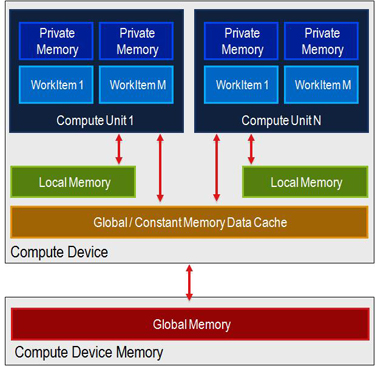
\includegraphics[width=70mm]{img/mem-cl.jpg}
\caption{OpenCL memory hierarchy.}
\label{cl-mem}
\end{figure}

\begin{itemize}
\item{{\bf Global Memory} - The global memory has the larget capacity and can be used by all work items. It is considered of being the slowest memory subsystem. The best performance is achieved when streaming contiguous memory addresses or patterns that can explore the full bandwidth (similar to the coalesced memory reads in CUDA). }
\item{{\bf Private Memory} - The memory used in a single work items. Can not be shared between work items. Similar to registers in GPU multiprocessors or CPU cores. The private memory is allocated and partioned at compile time. There is no maximum private memory size defined  in the OpenCL specification. Using too much private memory can lead to a slowdown since OpenCL will user slower memory spaces once the private memory is full.}
\item{{\bf Local Memory} - Local memory can be shared between work items in a work group, similar to the shared memory in the CUDA architechure. Local memory is used when data from global memory is needed and one wants to reduce the global memory reads within a work group.}
\item{{\bf Constant Memory} - Constant memory is implemented differently on certain deviced. For example, on NVIDIA GPU cards, the constant memory is located at region good for broadcasting. On ATI GPU cards, the constant memory is part of the global memory but with optimized broadcasting.}
\end{itemize}

\subsubsection{Work Groups}

Kernels are being executed over a 1D, 2D, 3D grid or NDRange. The kernel is then executed in parallel where each kernel instance is called work item. Work items are divided in work groups of the global grid. The developer can explicity set the size of the work group or let it be decided at runtime.

\renewcommand{\lstlistingname}{Code}
\begin{lstlisting}[caption= Example of vector addition in OpenCL, label=cl1]
__kernel void VectorAddition( __global float * A,
                              __global float * B,
                              __global float * C,
                              int width)
{ 
    const int x = get_global_id(0); 
    const int y = get_global_id(1); 
    const int idx = x + y * width;
    C[idx] = A[idx] + B[idx];
}
\end{lstlisting}

Code \ref{cl1} shows an example of a simple vector addition. Keyword \texttt{\_\_kernel} tells the compiler it is a OpenCL kernel and \texttt{\_\_global} specifices a pointer to the global memory space. Inside the kernel, the function \texttt{get\_global\_id} is used to find the horizontal and vertical id of the work item (this only works if the kernels are executed with a two dimensional work size).


\section{Implementation}


\section{Results}

\section{Discussion}
\subsection{Comparision between the GPU environments}


\subsection{OpenGL interoperability}

Currently, if an image has been created/modified with gpuip and needs to be display, it has to first be copied back to the CPU and then uploaded back to the GPU for viewing. Both OpenCL and CUDA supports OpenGL interoperability by mapping a GPU buffer to an OpenGL buffer. This means that data produced by OpenCL and CUDA can be used as an OpenGL texture without unnecessary transfering between the CPU and the GPU. Although more internal work, the public API for {\tt Buffer} would not change much:
\newline
\renewcommand{\lstlistingname}{Code}
\begin{lstlisting}[caption= gpuip OpenGL interoperability, label=glinter]
struct Buffer{
  // ... rest of Buffer declarations 
  bool glInteroperability;
  GLint glTexture;
};
\end{lstlisting}

I think this option would make the library more lucrative to use in applications that are using OpenGL for viewing graphics. One particular case I could see it being useful is in deferred rendering for realtime 3D graphics. Once geometry has been rendered to different textures, it might be faster to apply operations in OpenCL or CUDA than it is in GLSL (there is no support for sharing memory between execution threads in GLSL).

\subsection{Template kernels}

Consider a case where you only want to write one kernel file but support multiple fileformats. For GLSL, this is already true and quite practical. However, it is not possible in OpenCL and CUDA. CUDA supports templated functions. It would be possible to have the data types as template typenames and therefore only writing the kernel once if {\tt half} (16-bit floating point) computation was supported. In OpenCL, half computation is supported if the graphics drivers come with the {\tt cl\_khr\_fp16} extension. OpenCL does not support templates but since we parse the kernel code ourselves in gpuip, we could implement our own templating rules and generate one OpenCL kernel for every data type that gpuip supports. 

\subsection{Computations as input}

It is only possible to write data per pixel in gpuip. If an algorithm would require a global property of a buffer, like the maximum or average value, it would not be possible. For example, if someone wants to write a tonemapping algorithm, they might compute a tonemapping value per pixel and then use the average value of all pixels as input to a second step in the tonemapping. A kernel can have user-defined parameters but not parameters that depends on the output of a kernel. It might be nice to add an option to make it possible to use the computation of a buffer as input. To make things still fairly simple, it could be restricted to only allow computations of one-dimensional buffers. Then a computation could be operators such as min, max, median, avg and sum. Behind the scenes, gpuip would perform the gpu algorithms. For example, to get the minimum value of a one-dimensional buffer, it would have to run a reduce algorithm. It might be worth exploring the common libraries for the GPU computing. Using libraries like Boost Comput[ref] and Thrust[ref] would save time and probably have better performance.

\subsection{Work item distribution}

Some algorithms might be optimized further by allowing a work item/thread write to more than one pixel. For example, in separable blur algorithms, it might be worth splitting the algorithm in two steps and have each work item operate on a row/column alone. Memory lookups tend to be the expensive part of an algorithm and if a work item can work alone on a row, data could be stored in the local registers as the work item iterates over the pixels. The public API of gpuip could be changed to something like this.
\newline
\renewcommand{\lstlistingname}{Code}
\begin{lstlisting}[caption= gpuip kernel work item distribution, label=dist]
struct Kernel{
  // ... rest of Kernel declarations 
  enum WorkDistribution { PIXEL, ROW, COLUMN };
  WorkDistribution distribution;
};
\end{lstlisting}
A different work item distribution is not possible in GLSL where every kernel has to be executed on a per pixel level.


\begin{thebibliography}{9}
\addcontentsline{toc}{section}{References}

\bibitem{glshadinglanguage}
  R. J. Rost
  \emph{OpenGL Shading Language.}
  2nd Edition,
  2006.

\bibitem{cudaexample}
  J. Sanders, E. Kandrot
  \emph{CUDA By Example.}
  1st Edition,
  2010.

\bibitem{cudapguide}
  NVIDIA
  \emph {CUDA C Progamming Guide.}

  http://docs.nvidia.com/cuda/cuda-c-programming-guide/ [2014-06-23]



\end{thebibliography}


\end{document}
